% Section 3.4 -- storage sensing and risk rule (short form; the full description, scenarios and figures are in the repository:
% firmware/, layers/L3b_storage_iot/, paper/sections/_supplement_storage.tex).
\subsection{Storage Sensing and Risk Rule}
\label{sec:method-storage}

Figure~\ref{fig:node} shows the storage node and its data path. One protected SHT30 temperature and humidity
probe~\cite{sht3x} is placed in a bag of grain and read every five minutes by an ESP32 board~\cite{esp32}; readings are sent by Message Queuing Telemetry Transport (MQTT) with Transport Layer Security (TLS), kept in a 24-hour buffer until the server confirms it has stored each one
once, and assessed hourly. Grain balances its moisture with the air between the kernels, and that air's relative humidity divided by
100 is its water activity $a_w$. Storage fungi need at least 65\,\% relative humidity (RH)~\cite{gwinner1996}, and grain below 65 to 70\,\% degrades slowly~\cite{delucia1994}. The rule takes the median
humidity and temperature of the last 24\,h and returns LOW for $a_w<0.65$, MEDIUM for $0.65\le a_w<0.70$ and HIGH from $0.70$; the
level rises at once but falls only after 48\,h at least 2 points below the limit; it returns UNKNOWN, with reasons, when the probe
hangs in shed air, in the first 6\,h, or when readings are old or missing. It says whether the air in a bag favors mold and insects;
it does not measure moisture content or detect spoilage. The firmware runs unchanged on a Wokwi twin with an emulated SHT3x
sensor~\cite{wokwi}, and the planner gives at-risk lots the earliest dates.

\begin{figure}[t]
  \centering
  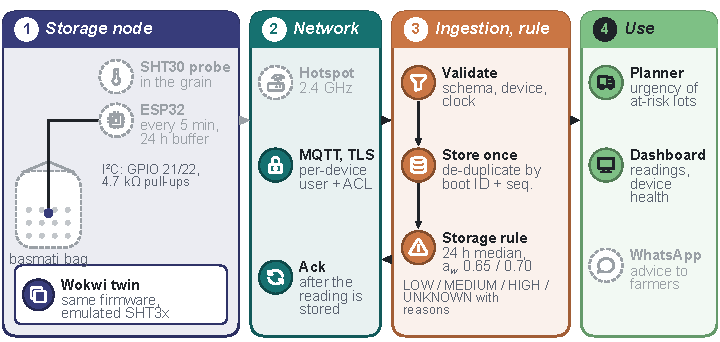
\includegraphics[width=\textwidth]{fig3_hardware.pdf}
  \caption{Storage node and data path. The ESP32 reads the probe in the grain (1) and sends each reading over MQTT with TLS (2); the
  server validates it, stores it once and applies the storage rule (3); and the planner and the manager app use the result (4). The
  firmware runs on a Wokwi twin~\cite{wokwi}; dashed grey parts (the physical probe, board and hotspot, and storage advice on
  WhatsApp) are the field deployment. ACL: access control list; I\textsuperscript{2}C: inter-integrated circuit bus; GPIO:
  general-purpose input/output.}
  \label{fig:node}
\end{figure}
